\section{Introduction}
\label{sec:intro}


% 为了全面评估LLMs日益增强的代码生成能力，研究界已提出了诸多代码生成基准（Benchmarks）。从早期的HumanEval和MBPP，到近期涌现的LiveCodeBench和FullStackBench，代码生成基准正朝着更高难度、更复杂的任务场景以及更贴近实际应用的方向发展。然而，现有基准普遍采用人工或半人工标注的方式构建，这带来了显著挑战。首先，人工标注的固有低效性和高昂成本，使其难以适应LLMs快速发展和迭代的需求，从而限制了高质量、大规模评估数据集的构建。其次，随着LLMs能力的提升，现有基准中较简单的编程任务已不足以充分反映当前模型的代码生成能力。这些局限性使得现有基准难以同时实现高难度、多语言支持及全面性评估（如图1所示）。
%To evaluate the rapidly advancing code generation capabilities of LLMs, a growing number of benchmarks have been introduced.

%As LLMs become increasingly capable, it becomes crucial to develop reliable benchmarks that can comprehensively evaluate their code generation performance. 


Recently, Large Language Models (LLMs) have undergone rapid development, demonstrating impressive capabilities in various tasks~\citep{gpt4o,gemini2.5,deepseekai2025deepseekr1,tencenthunyuanteam2025hunyuanturbos}. Among these, code generation has emerged as a key indicator of both model intelligence and practical utility, attracting growing attention from both academia and industry~\citep{chen2021evaluatinglargelanguagemodels,jimenez2024swebench,jiang2024surveylargelanguagemodels}. By generating executable code, LLMs have the potential to significantly enhance programming automation and alleviate the burden of manual coding. Many popular and powerful LLMs like Claude 4~\citep{claude4} and DeepSeek-V3~\citep{deepseek_v3} have already been widely adopted in AI-assisted coding scenarios~\citep{Cursor}.



To measure and improve the code generation capabilities of LLMs, numerous code generation benchmarks are proposed~\citep{wang2025softwaredevelopmentlifecycle}. Early works such as HumanEval~\citep{chen2021evaluatinglargelanguagemodels} and MBPP~\citep{austin2021programsynthesislargelanguage} laid the foundation by evaluating LLMs' abilities on short, algorithm-focused Python problems. However, these simple and narrowly defined tasks have quickly become outdated with the rapid development in LLMs. Recent benchmarks~\citep{quan2025codeelobenchmarkingcompetitionlevelcode,jain2025livecodebench,zheng2025livecodebenchproolympiadmedalists,zhu2025oibenchbenchmarkingstrongreasoning} have shifted focus to more challenging, competition-level Python problems with the help of professional manual annotations. %For example, LiveCodeBench~\citep{jain2025livecodebench} periodically collects manually written Python competition problems to construct a contamination-free benchmark. 
On the other hand, some other benchmarks~\citep{peng2024humanevalxlmultilingualcodegeneration,chai2025mceval,fullstackbench}, such as FullStackBench~\citep{fullstackbench}, emphasize more practical multilingual programming scenarios. However, manually crafting these programming problems and test cases is time-consuming and labor-intensive, making it difficult to simultaneously achieve high difficulty and multilingual coverage, as shown in Table~\ref{introduction_benchmark}. \textbf{\textit{Therefore, the community currently needs a benchmark that combines high difficulty, practical diversity, and balanced multilingual distribution to comprehensively evaluate the code generation capabilities of LLMs.}}
%This makes it challenging to comprehensively evaluate the full potential of LLMs. \textbf{\textit{To date, no code generation benchmark has achieved a combination of high difficulty, practical diversity, and balanced multilingual coverage}}.






\begin{table}[]
\small
\resizebox{\textwidth}{!}{
\begin{tabular}{lcccccccc}
\toprule
\textbf{Benchmark} & \textbf{MLing} & \textbf{MLogi} & \textbf{HFree} & \textbf{BDist} & \textbf{Difficulty} & \textbf{Category} & \textbf{Data Size} & \textbf{Problem Len}  \\ \midrule
HumanEval          & 
\includegraphics[width=0.35cm]{./figures/no.png}                & 
\includegraphics[width=0.35cm]{./figures/no.png}                  & 
\includegraphics[width=0.35cm]{./figures/no.png}              & /    & 
\includegraphics[width=0.25cm]{./figures/star.png}                    & \textcolor{gray!80!black}{5} & \textcolor{gray!80!black}{164}                & \textcolor{orange!80!black}{134.1}                    \\
MBPP               & 
\includegraphics[width=0.35cm]{./figures/no.png}                    & 
\includegraphics[width=0.35cm]{./figures/no.png}                  & 
\includegraphics[width=0.35cm]{./figures/no.png}               & /    & 
\includegraphics[width=0.25cm]{./figures/star.png}                   &  \textcolor{gray!80!black}{6} & \textcolor{gray!80!black}{378}                & \textcolor{gray!80!black}{50.5}                     \\
BigCodeBench       & 
\includegraphics[width=0.35cm]{./figures/no.png}                    & 
\includegraphics[width=0.35cm]{./figures/no.png}                  & 
\includegraphics[width=0.35cm]{./figures/no.png}                & /    & 
\includegraphics[width=0.25cm]{./figures/star.png}
\includegraphics[width=0.25cm]{./figures/star.png}
\includegraphics[width=0.25cm]{./figures/star.png}                 &  \textcolor{orange!80!black}{8} & \textcolor{orange!80!black}{1140}               & \textcolor{orange!80!black}{146.7}                    \\
LiveCodeBench      & 
\includegraphics[width=0.35cm]{./figures/no.png}                    & 
\includegraphics[width=0.35cm]{./figures/no.png}                  & 
\includegraphics[width=0.35cm]{./figures/no.png}               &  /     & 
\includegraphics[width=0.25cm]{./figures/star.png}
\includegraphics[width=0.25cm]{./figures/star.png}
\includegraphics[width=0.25cm]{./figures/star.png}
\includegraphics[width=0.25cm]{./figures/star.png}
\includegraphics[width=0.25cm]{./figures/star.png}               &  \textcolor{gray!80!black}{4} & \textcolor{orange!80!black}{1100}               & \textcolor{green!80!black}{469.6}                    \\
FullStackBench     & 
\includegraphics[width=0.35cm]{./figures/yes.png}                   & 
\includegraphics[width=0.35cm]{./figures/no.png}                  & 
\includegraphics[width=0.35cm]{./figures/no.png}              &   
\includegraphics[width=0.35cm]{./figures/no.png}    & 
\includegraphics[width=0.25cm]{./figures/star.png}
\includegraphics[width=0.25cm]{./figures/star.png}                  &  \textcolor{green!80!black}{12} & \textcolor{orange!80!black}{1687}               & \textcolor{orange!80!black}{184.3}                    \\
McEval             & 
\includegraphics[width=0.35cm]{./figures/yes.png}                   & 
\includegraphics[width=0.35cm]{./figures/no.png}                  & 
\includegraphics[width=0.35cm]{./figures/no.png}         & 
\includegraphics[width=0.35cm]{./figures/yes.png}         & 
\includegraphics[width=0.25cm]{./figures/star.png}
\includegraphics[width=0.25cm]{./figures/star.png}                  &  \textcolor{orange!80!black}{9} & \textcolor{green!80!black}{2007}               & \textcolor{orange!80!black}{146.7}                    \\ \midrule
\textbf{AutoCodeBench}      & 
\includegraphics[width=0.35cm]{./figures/yes.png}                   & 
\includegraphics[width=0.35cm]{./figures/yes.png}                 & 
\includegraphics[width=0.35cm]{./figures/yes.png}             & 
\includegraphics[width=0.35cm]{./figures/yes.png}    & 
\includegraphics[width=0.25cm]{./figures/star.png}
\includegraphics[width=0.25cm]{./figures/star.png}
\includegraphics[width=0.25cm]{./figures/star.png}
\includegraphics[width=0.25cm]{./figures/star.png}
\includegraphics[width=0.25cm]{./figures/star.png}               &  \textbf{\textcolor{green!80!black}{14}} & \textbf{\textcolor{green!80!black}{3920}}               & \textbf{\textcolor{green!80!black}{498.2}} \\ 
\bottomrule
\end{tabular}
}
\caption{Comparison of Existing Code Generation Benchmarks and AutoCodeBench. \textbf{MLing}: MultiLingual; \textbf{MLogi}: MultiLogical, refers to programming problems that require the model to simultaneously implement multiple core functionalities. \textbf{HFree}: Human-Free; \textbf{BDist}: Balanced Distribution of multiple languages. The \textbf{Difficulty} is rated based on the performance of \texttt{DeepSeek-V3-0324}. The number of \textbf{Category} is obtained using predefined labels from \texttt{DeepSeek-V3-0324}. The \textbf{Problem Len}gth is calculated using \texttt{Qwen2.5-32B-Instruct} tokenizer.}
\label{introduction_benchmark}
\end{table}




%In this paper, we explore automating the synthesize of code generation benchmarks without any manual annotations. 
%While previous works~\citep{wei2024magicoder,luo2024wizardcoder,NEURIPS2024selfcodealign,wu2024inversecoder,xu2025kodcode} for synthesizing code generation data, they are not suitable for creating benchmark due to insufficient accuracy. 
In this paper, we propose \textbf{AutoCodeGen}, an automated workflow centered around LLM-Sandbox Interaction, to accurately synthesize high-difficulty multilingual code generation datasets without any manual annotations. Unlike previous data synthesis strategies~\citep{luo2024wizardcoder,magicoder,xu2025kodcode,li2025codeio}, we ensure high data quality by constructing multilingual sandbox to generate test outputs and synthesizing programming problems in reverse order. Concretely, AutoCodeGen consists of the following key steps: 1) \textbf{Solution Generation}: Based on real-world code snippets, LLMs evolve self-contained code solutions, ensuring their practicality and diversity. 2) \textbf{Test Function Generation}: LLMs generate test inputs, which are concatenated with the code solutions and executed in the sandbox to obtain the test outputs. The two are then combined to form a complete test function. Compared to directly generating complete test cases as in KodCode~\citep{xu2025kodcode} or using Input Generator~\citep{li2025codeio}, our method efficiently ensures the correctness and completeness of the test cases. 3) \textbf{Problem Generation}: LLMs generate challenging programming problems based on heuristic specifications and integrates public test cases into them. 4) \textbf{Filtering}: Finally, we filter the data by Multiple Sampling, LLM-as-Critic, and Tagging to maintain the high-difficulty, high-quality, and diversity. 

Based on the automation workflow mentioned above, we propose \textbf{AutoCodeBench}, a large-scale, human-free code generation benchmark featuring 3,920 problems, as shown in Table~\ref{introduction_benchmark}. Compared with previous multilingual benchmarks~\citep{cassano2022multiplescalableextensibleapproach,fullstackbench,chai2025mceval}, ours simultaneously offers high difficulty, diversity, and practicality, with a balanced distribution of problems across 20 programming languages. Besides, we intentionally include multi-logical problems to assess the LLMs' ability to handle multi-logical reasoning. We believe this capability is important in the code agents scenarios like SWE-Bench~\citep{jimenez2024swebench}. 
%There is experimental results and analysis.

The key contributions of this paper are as follows:






\begin{enumerate}
    \item \textbf{AutoCodeGen}. We propose an automated workflow based on LLM-Sandbox Interaction, where LLMs generate test inputs and obtain test outputs through the sandbox, to create high-quality code generation benchmarks. Worth mentioning is that this workflow can also be applied to synthesize high-quality training data.
    \item \textbf{AutoCodeBench}. We introduce AutoCodeBench, a large-scale code generation benchmark with 3,920 problems, evenly distributed across 20 programming languages, featuring high-difficulty, practicality, and diversity. Based on the evaluation results, we construct a simplified version AutoCodeBench-Lite. Besides, We tailor AutoCodeBench-Complete, a completion-based code generation benchmark, to assess the performance of base models.
    \item \textbf{Multilingual Sandbox}. We open-source a sandbox that supports 20+ programming languages. It is capable of high concurrency and request-based calls, making it suitable for multilingual evaluation and large-scale training.
    \item \textbf{Experimental Results}. We evaluate 30+ open-source and proprietary models. The results show that even the most advanced LLMs still struggle with complex and diverse multilingual programming tasks, especially in multi-logical scenarios.
    \item \textbf{Data and Experiment Analysis}. We conduct a comprehensive analysis of AutoCodeGen and AutoCodeBench, focusing on key aspects such as the quality, difficulty, and diversity of the generated data, as well as potential model biases during the generation process. We hope that these insights can provide valuable experience for the community in the development of future code generation benchmarks.
\end{enumerate}





% 我们在20种编程语言上应用该方法，构建了AutoCodeBench，一个无需人工标注的多语言、高难度、真实且多样的代码生成Benchmark。



% 在这篇论文中，我们探索了使用大模型自动构建代码生成benchamrk，来摆脱人工标注。我们的方法分为如下几步：1）从预训练数据中收集大量的代码片段作为种子，来保证真实性与多样性；2）基于种子进化出自包含的代码答案，并在LLM-Sandbox的多次交互中合成测试函数，保证了数据的准确性；3）提示LLM基于代码和测试函数生成编程问题；4）使用LLM多次采样和打标的方式筛选数据，保证了数据的难度和多样性。





% 基于真实的代码片段合成，保证实际性；
% LLM-Sandbox交互，保证正确性；
% 调用LLM对每道编程问题多次采样，并根据通过次数过滤数据，保证了难度；
% LLM-as-a-Critic对题目和测试函数做check，保证了题目的质量；
% 设计多样性打标抽样策略保证数据的多样性。


 

% 为了应对上述挑战，本论文深入探索了一种利用大模型自动构建代码生成基准的方法，旨在免除对人工标注的依赖。我们提出了一种基于LLM-Sandbox交互的工作流：首先，从大规模预训练代码语料库中抽取函数级、类级和文件级的真实且多样的代码种子；随后，基于这些种子提示LLM演化出独立的、自包含的代码片段；紧接着，我们通过LLM与沙盒环境的多次迭代交互来构建全面且正确的测试函数。为了精准控制编程问题的难度和生成质量，我们分别采用了LLM多次采样和LLM-as-Critic的策略。最终，我们对生成数据进行打标抽样来确保基准的多样性。

 

% 通过上述全自动化的工作流，我们成功构建了AutoCodeBench——一个包含20种编程语言、编程指令足够复杂且多样的代码生成基准。我们在20多个开源和闭源模型上进行了全面评测，结果显示AutoCodeBench具有较高的任务难度和良好的模型区分度，并清晰揭示了当前模型在面对多语言复杂编程指令时所存在的不足。此外，我们通过人工抽样方式对自动化生成内容的准确性进行了评估，结果表明我们方法的准确率达到了92%以上。

 

% 我们的主要贡献如下：

% 我们提出了利用大模型自动构建代码生成基准的方法，并构建了一套创新的LLM-Sandbox交互式工作流。这代表了大模型代码能力自我评估（self-evaluation）领域的一次全新尝试。

% 我们提出了AutoCodeBench，一个无需人工生成的代码生成基准集，其显著特点在于高难度的复杂编程指令和广泛的多语言覆盖。

% 实验结果明确揭示了当前大模型在解决高难度、多语言复杂编程问题方面的能力瓶颈，这为未来大模型代码能力的提升指明了关键研究方向。


\section{AutoCodeBench: A Challenging, Practical, and Diverse Multilingual Benchmark}

In this section, we first provide an overall data statistics of the AutoCodeBench and its simplified version AutoCodeBench-Lite. Following this, we introduce the automated workflow, AutoCodeGen, used to generate AutoCodeBench(-Lite). 

\subsection{Data Overview}

As shown in Table~\ref{introduction_benchmark} and ~\ref{method_bench}, AutoCodeBench is a large-scale, high-difficulty multilingual benchmark. Over 60\% of the problems are classified as hard problems, with each problem averaging 498.2 characters and accompanied by 9.6 test cases, providing a challenging and comprehensive evaluation standard. The 20 languages are as follows: \textit{Python, C++, Java, JavaScript(JS), Go, Shell, C\#, Dart, Elixir, Julia, Kotlin, Perl, PHP, Racket, R, Ruby, Rust, Scala, Swift, TypeScript(TS)}. 
% AutoCodeBench-Lite is a simplified subset of AutoCodeBench.





To analyze the diversity and language coverage of AutoCodeBench, we first use \texttt{Claude Sonnet 4} to generate 20 language-agnostic task categories, and then employ \texttt{DeepSeek-V3-0324} to classify each problem accordingly. Categories with less than 2\% representation are merged into the ``Other'' group. As shown in Figure~\ref{fig:statistic_acb}, AutoCodeBench covers 14 categories, demonstrating comprehensive coverage of practical programming scenarios. Besides, we analyze the distribution of problems across the 20 programming languages. AutoCodeBench exhibits a relatively balanced distribution across languages, with no significant bias toward any specific one, further validating its completeness and representativeness as a multilingual benchmark. Category labels and statistics of other benchmarks are provided in Appendix~\ref{appendix:a}.
%The statistics of AutoCodeBench-Lite and other benchmarks are provided in the appendix.



\begin{table}[]
\begin{tabular}{lcccccc}
\toprule
                   & \#Problems & \#Test Cases & \#Langs & Prob Len  & Solu Len & Difficulty (Easy/Med/Hard) \\
\midrule
ACB      & 3,920      & 37,777       & 20          & 498.2                & 487.5                 & 646/846/2428                    \\
ACB-Lite &   1,586         &  15,341            &    20         &                     517.2         &                          469.3     & 263/421/902  \\
\bottomrule
\end{tabular}
\caption{Statistics of ACB and ACB-Lite. \textbf{ACB}: AutoCodeBench; \textbf{Langs}: Languages; \textbf{Prob}: Problem; \textbf{Solu}: Solution; \textbf{Len}: Length; \textbf{Med}: Medium. The difficulty level is determined by the number of passes in ten samplings of \texttt{DeepSeek-Coder-V2-Lite}. Problems with zero correct solutions are classified as hard, 1-5 correct solutions as medium, and those with more than five as easy.}
\label{method_bench}
\end{table}






\begin{figure}[t]
\centering
\begin{subfigure}[b]{0.45\textwidth}
    \centering
    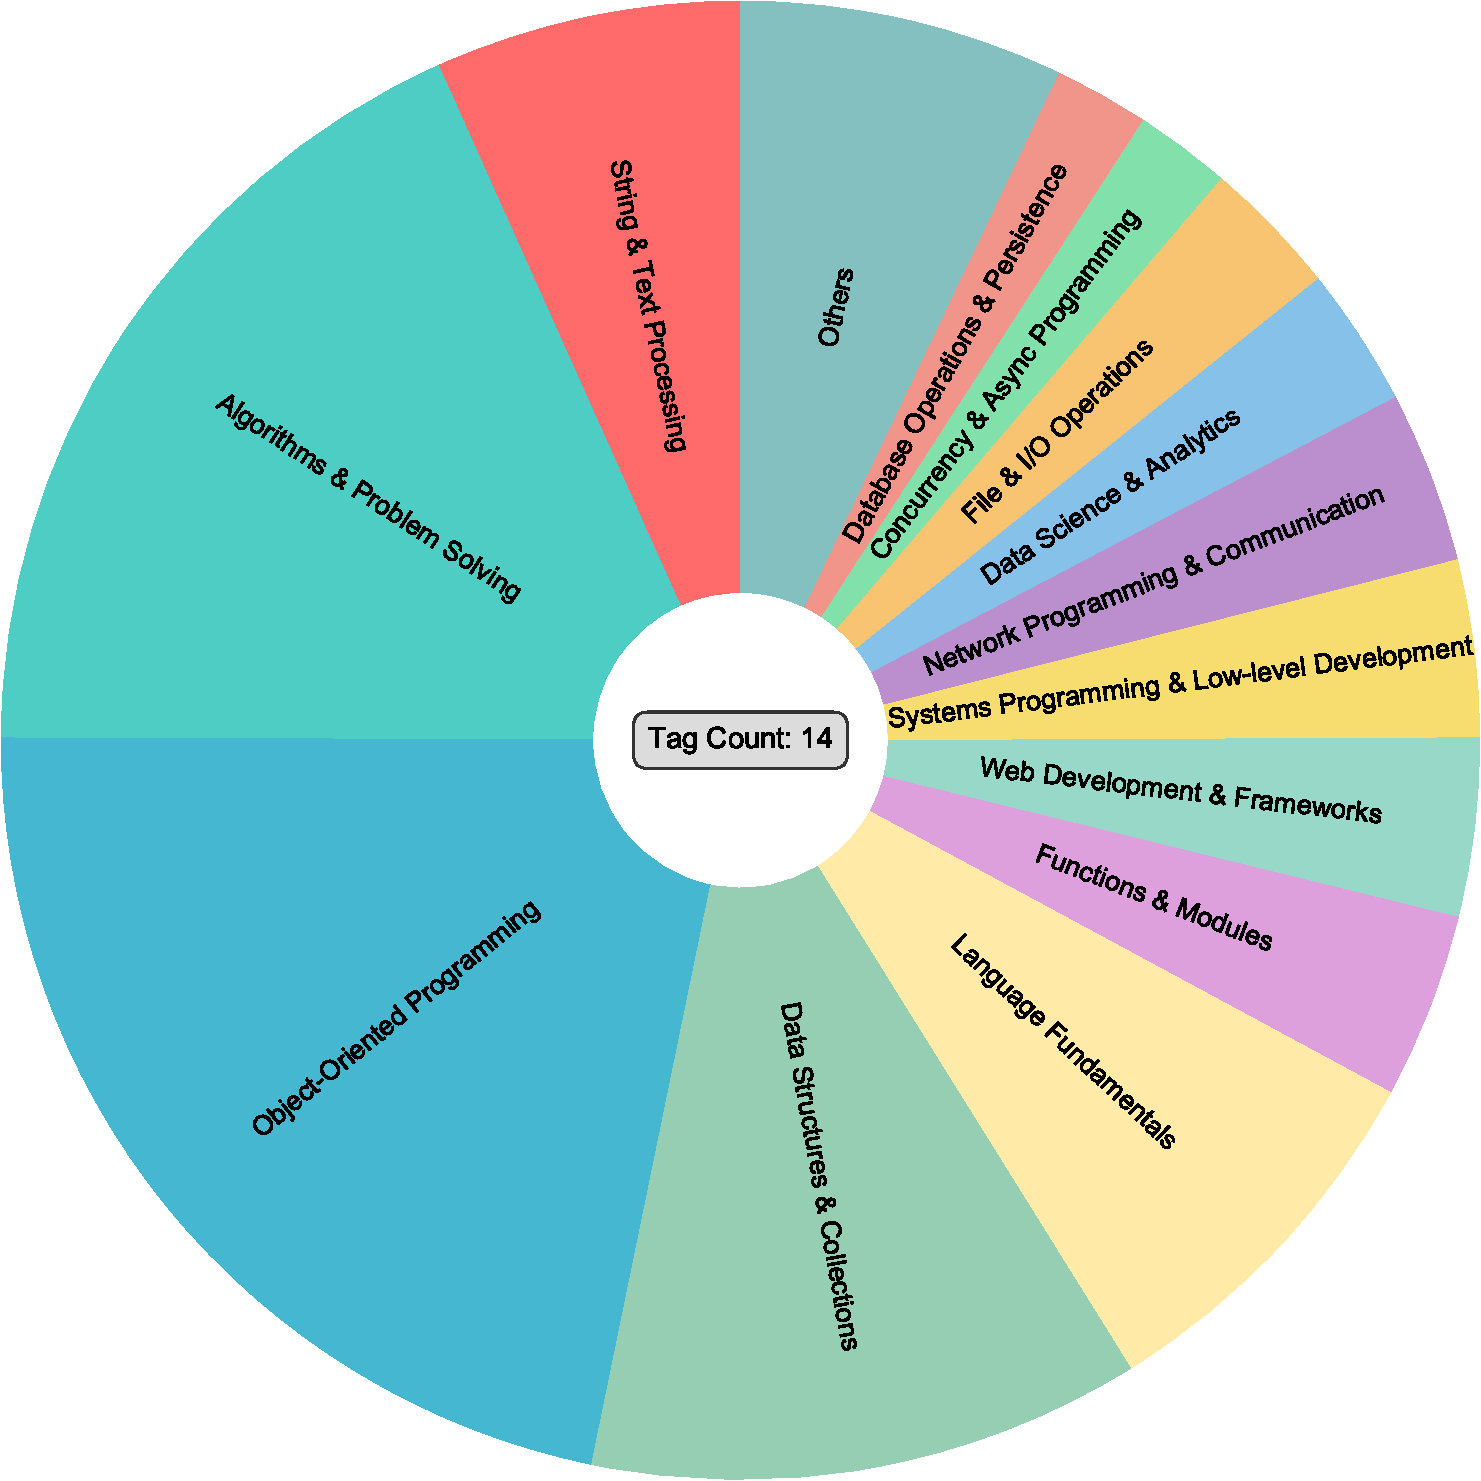
\includegraphics[width=\textwidth]{figures/tag_acb.pdf}
    \label{fig:tag_acb}
\end{subfigure}
\hfill
\begin{subfigure}[b]{0.45\textwidth}
    \centering
    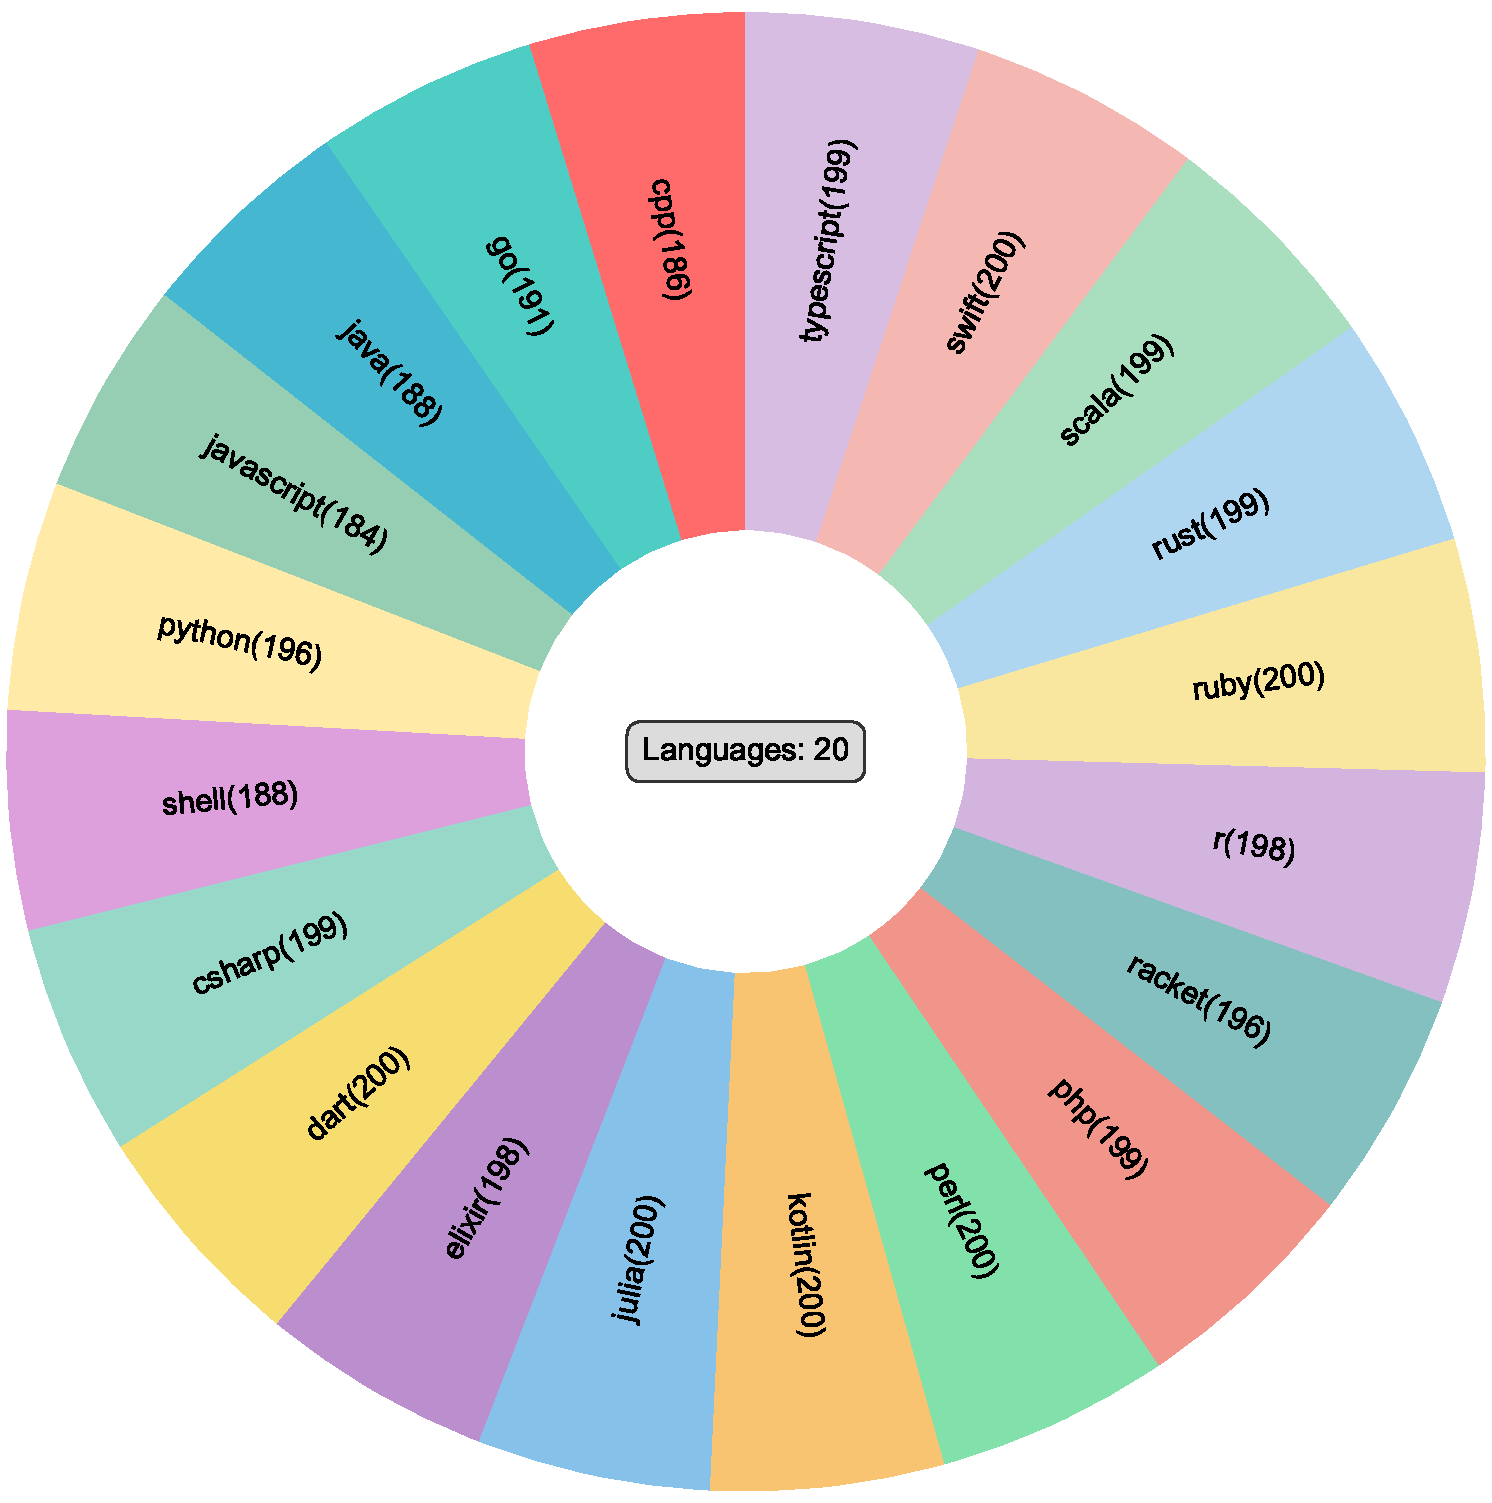
\includegraphics[width=\textwidth]{figures/lan_acb.pdf}
    \label{fig:lan_acb}
\end{subfigure}

\caption{Tag and Language Distribution across our AutoCodeBench.}
\label{fig:statistic_acb}
\end{figure}




\subsection{Automated Workflow}



\begin{figure*}[t]
    \centering
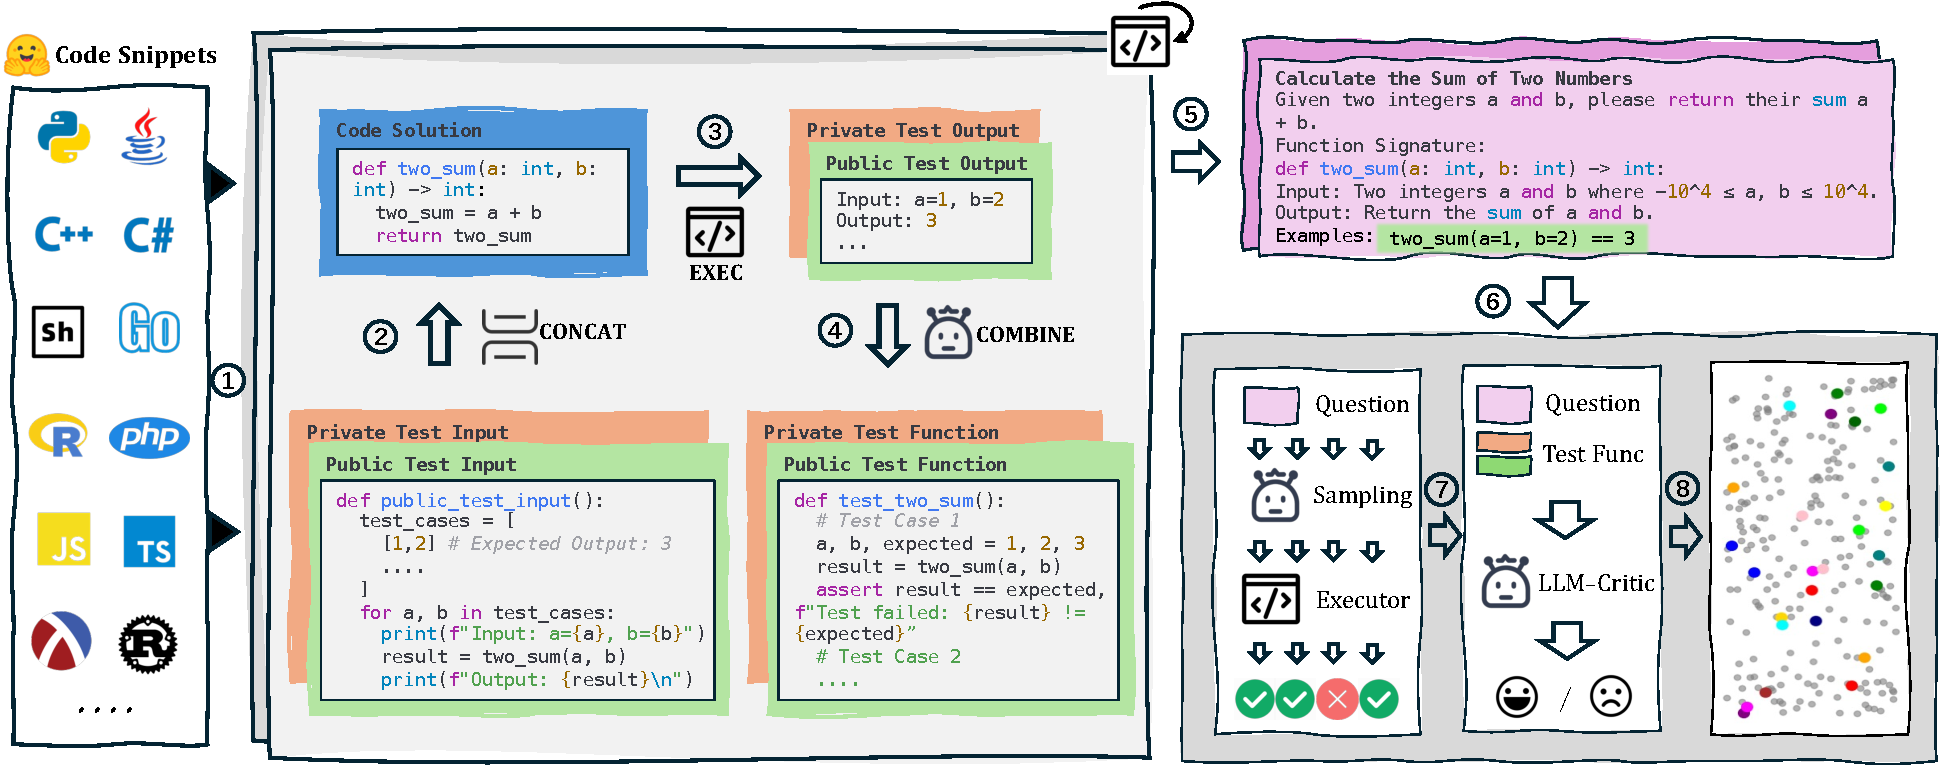
\includegraphics[width=1.0\columnwidth]{figures/workflow.pdf}
    \caption{\textbf{The overview of AutoCodeGen}. It first generates code solution and the corresponding public/private test input functions based on multilingual code snippets (\textcircled{1}). They are concatenated and executed in a sandbox to obtain test outputs, which are then combined by the LLM into complete test functions (\textcircled{2},\textcircled{3},\textcircled{4}). Based on the code solution and test function, the LLM is prompted to generate accurate programming problems (\textcircled{5}). Finally, a three-stage data filtering is applied: multiple sampling to remove too easy problems (\textcircled{6}), LLM-as-Critic to discard low-quality ones (\textcircled{7}), and diversity-based tagging to ensure distributional variety (\textcircled{8}).}
	\label{method:workflow}
\end{figure*}

% Our workflow for constructing code generation benchmarks consists of a fully automated pipeline, designed to produce high-quality, diverse, and challenging programming problems, as illustrated in Figure~\ref{method:workflow}. The process includes four key stages: Code Solution Generation (\textcircled{1}), Test Function Generation (\textcircled{2},\textcircled{3},\textcircled{4}), Programming Problem Generation (\textcircled{5}), and Data Filtering (\textcircled{6},\textcircled{7},\textcircled{8}).
Our AutoCodeGen based on LLM-Sandbox interaction for constructing code generation benchmarks is fully automated. It first generates large-scale multilingual data with guaranteed executability and correctness, then applies a three-stage filtering strategy to ensure the benchmark is challenging, high-quality, and diverse. As illustrated in Figure~\ref{method:workflow}, the workflow includes four key stages: \textbf{Code Solution Generation} (\textcircled{1}), \textbf{Test Function Generation} (\textcircled{2},\textcircled{3},\textcircled{4}), \textbf{Programming Problem Generation} (\textcircled{5}), and \textbf{Data Filtering} (\textcircled{6},\textcircled{7},\textcircled{8}).


%The core advantage strength of our workflow lies in its reverse-order problem construction and the use of LLMs to generate test inputs, which are executed in a sandbox to obtain test outputs—ensuring factual correctness and consistency. Additionally, our multi-stage data filtering strategy guarantees the resulting dataset is of high quality, diverse, and challenging.











\subsubsection{Code Solution Generation}

We begin by extracting multilingual code snippets from Stack-Edu~\citep{allal2025smollm2smolgoesbig}, a large-scale dataset of educational code filtered from The Stack v2~\citep{lozhkov2024starcoder}, as seeds. These seeds span function-level, class-level, and file-level code, sourced from real GitHub repositories, ensuring diversity and practicality. Using a language-specific few-shot prompt, we guide \texttt{DeepSeek-V3-0324} to refine and evolve these seeds into verifiable and self-contained code solutions. During this process, the model removes non-essential logic and adds appropriate comments for clarity. We then validate the correctness of the generated solutions by multilingual sandbox.

\subsubsection{Test Function Generation}

% Different from LLM-generated test case or Input Generator method, we first generate test input functions using 

% Previous test case generation methods either directly relied on LLM-generated outputs or used Input Generators like CodeI/O to automate test case creation. However, these methods faced limitations in test output generation and edge case coverage. To balance efficiency and comprehensiveness, our method involves generating test input functions using LLM, then combining them with the code solution to generate the test output.

We enhance efficiency and edge-case coverage by first generating test inputs via LLMs and then executing them in a sandbox to obtain the corresponding outputs. Specifically, Test Function Generation is divided into the following three steps:

\textbf{Test Input Generation} The test input functions (both public and private) are generated alongside the above code solution, ensuring alignment between the solution and its inputs. The public test input function includes no more than 3 basic cases and serves demonstration purposes; it will be embedded into the final programming problem as an illustrative usage. In contrast, the private test input function contains 7+ inputs, including edge cases, and functions as the comprehensive test for verifying the correctness of the code solution.

\textbf{Test Output Generation} We concatenate the code solution with test input functions and execute them in the sandbox to obtain the corresponding test outputs.

\textbf{Input-Output Integration} We prompt \texttt{DeepSeek-V3-0324} with both the test input functions and output results to generate coherent and verifiable test functions. Finally, we validate the correctness by executing the code solution together with the generated public and private test functions in the sandbox.

\subsubsection{Programming Problem Generation} 
\label{method_probelm_generate}

Generating high-quality programming problems is challenging, as it requires detailed and accurate problem descriptions. We find that models often omit key information when generating programming problems, such as the entry point specified in the test function. Therefore, we define a set of specifications that generated problems must meet:

\begin{itemize}
    \item Language Specification: Explicitly states the programming language to be used.
    \item Problem Description: A precise and unambiguous description of the task.
    \item Function/Class Naming: Clear identification of all functions and classes involved in the test function.
    \item Input/Output Format: Explicit definitions of input and output types and value ranges.
    \item Example Usage: Provides sample tests embedded with the generated public test functions for reference.
    \item No Solution Hints: The problem description must not include hints to the solution.
\end{itemize}


Using these guidelines, we prompt \texttt{DeepSeek-V3-0324} to generate high-quality programming problems based on the code solution (with appropriate comments) and the corresponding test function, while embedding the public test function as example usage. 

\textbf{Through these three steps, we obtain a large-scale multilingual dataset, where each instance is represented as a tuple \textless{}programming problem, code solution, public test function, private test function\textgreater{}.}






\begin{table}[t]
\small
\centering
\begin{tabular}{cc|cc|cc|cc|cc}
\toprule
\textbf{Origin} & \textbf{Target} & \textbf{Origin} & \textbf{Target} & \textbf{Origin} & \textbf{Target} & \textbf{Origin} & \textbf{Target} & \textbf{Origin} & \textbf{Target} \\ \midrule
 Python          &  R &  Python          &  Ruby  & Java          &  Scala  & Java          &  C\#  &Shell          &  Perl \\
Python          &  Elixir  &Python          &  Julia    & Java         &  Kotlin & JavaScript          &  PHP & C++ & Rust \\ Python          &  Swift   & Python          &  Racket & Java & Dart   &  JavaScript        &  Typescript  \\
\bottomrule
\end{tabular}
\caption{Programming language translation pairs.}
\label{method:translate}
\end{table}






\subsubsection{Data Filtering}
\label{method_data_filtering}

Finally, We apply three filtering and sampling steps to ensure the \textbf{high-difficulty}, \textbf{high-quality}, and \textbf{diversity} of the final benchmark.

\textbf{Difficulty Control} Programming problems that are too simple are not meaningful for evaluating the code generation capabilities of current LLMs. To address this, we employ a moderately capable code model, \texttt{DeepSeek-Coder-V2-Lite}, to filter out too easy problems. Specifically, we sample answers for each problem ten times using the model and validate the correctness via sandbox execution. Problems that are solved correctly in all ten attempts are discarded. Take Python as an example, \texttt{DeepSeek-Coder-V2-Lite} can filter out 25.1\% of overly simple problems.

\textbf{Quality Control} During the aforementioned problem generation stage, we define six specifications to guide the generation of detailed and accurate programming problems. To further ensure high quality, we employ \texttt{DeepSeek-R1-0528} to critique each \textless{}problem, test function\textgreater{} pair. Specifically, assuming the problem is entirely correct, we evaluate the test function’s consistency with problem based on the following seven concepts:
\begin{itemize}
    \item Whether the function/class names or signatures match the problem description.
    \item Whether the test cases involve randomness or are non-reproducible.
    \item Whether the testing objective aligns with the stated purpose of the problem.
    \item Whether numerical precision is handled appropriately.
    \item Whether exception handling is used in a way that invalidates the test cases.
    \item Whether the test cases check for requirements beyond the problem description.
    \item Whether the test cases are comprehensive.
\end{itemize}


\textbf{Diversity Sampling}
We aim for our benchmark to cover as many real-world scenarios as possible. To this end, we perform diversity-based sampling on the existing data to construct the final benchmark. We use \texttt{DeepSeek-V3-0324} to label each problem. We then divide the problems into different pools by category and perform cyclic sampling, ensuring a broad representation of programming scenarios.



\subsubsection{Approximate Language Translation}

For Python, C++, Shell, Java, JavaScript, and Go, we directly use the workflow described above. For the other 14 languages, while the proposed workflow is still applicable, we choose to employ an approximate language translation approach due to their limited data resources and lack of diversity. We extract unused data from the data pool generated in Section~\ref{method_probelm_generate} and translate them into the target low-resource language, as shown in Table~\ref{method:translate}. This ensures a sufficient and diverse dataset, which is further refined through the Data Filtering process, as described in Section~\ref{method_data_filtering}.






\subsubsection{AutoCodeBench-Lite Construction}

To facilitate quicker and more efficient model evaluations, we create the AutoCodeBench-Lite, a simplified subset of AutoCodeBench.
%Specifically, AutoCodeBench-Lite is constructed by extracting the union of all the problems that every model is able to solve correctly from the evaluation results on AutoCodeBench. This curated subset provides a more lightweight benchmark, allowing for faster testing while still maintaining a representative set of problems that models can tackle.
Specifically, we collect the problem-solving results from all models and sort the problems in ascending order based on the number of passes. After discarding problems with fewer than 2 passes, we select approximately 1,500 problems based on their pass count in ascending order. These problems, which have been solved correctly by existing models at least twice and have a certain level of difficulty, are selected to amplify the differences between the models. We use these problems as the set for the Lite version.



